\documentclass[14pt]{extarticle}

\usepackage[table]{xcolor}
\usepackage{amsmath,mathtools,amsfonts,amsthm,amssymb,hyperref,wasysym,pifont}
\usepackage{parskip,geometry,latexsym,bookmark,mathtools,float,cancel,tcolorbox}

% for the Power set P
\usepackage[mathscr]{euscript}
\let\euscr\mathscr 
\let\mathscr\relax
\usepackage[scr]{rsfso}
\newcommand{\ps}{\mathscr{P}}

\newtheorem{defn}{Definition}
\newtheorem{thm}{Theorem}
\newtheorem{claim}{Claim}
\newtheorem{lemma}{Lemma}

\renewcommand{\arraystretch}{1.3}

\newcommand{\es}{\varnothing}
\newcommand{\dps}{\displaystyle}
\newcommand{\fbl}{\underline{\hspace{1cm}}\,\,}
\newcommand{\R}{\mathbb{R}}
\newcommand{\Z}{\mathbb{Z}}
\newcommand{\from}{\leftarrow}
\newcommand{\true}{{\bf t}}
\newcommand{\false}{{\bf c}}
\newcommand{\bic}{\leftrightarrow}
\newcommand{\base}[1]{{\color{cyan}#1}}
\newcommand{\floor}[1]{{\left\lfloor#1\right\rfloor}}
\newcommand{\ceil}[1]{{\lceil#1\rceil}}
\newcommand{\da}{\downarrow}
\newcommand{\fa}{\forall}
\newcommand{\te}{\exists}
\newcommand{\cy}{\color{cyan}}

\newcommand{\colsq}[1]{{\color{#1} $\blacksquare$}}

\newcommand\Ccancel[2][black]{\renewcommand\CancelColor{\color{#1}}\cancel{#2}}
\newcommand\Cbcancel[2][black]{\renewcommand\CancelColor{\color{#1}}\bcancel{#2}}

\hypersetup{colorlinks,allcolors=blue,linktoc=all}
\geometry{a4paper}
\geometry{margin=0.42in}

\title{Chapter 6 Solutions, Susanna Epp Discrete Math 5th Edition}

\author{https://github.com/spamegg1}

\begin{document}
\maketitle
\tableofcontents

\section{Exercise Set 6.1}

\subsection{Exercise 1}
In each of (a)–(f), answer the following questions: Is \(A \subseteq B\)? Is \(B \subseteq A\)? Is either $A$ or $B$ a 
proper subset of the other?

\subsubsection{(a)}
\(A = \{2, \{2\}, (\sqrt{2})^2\}, B = \{2, \{2\}, \{\{2\}\}\}\)

\begin{proof}
\(A = \{2, \{2\}, (\sqrt{2})^2\} = \{2, \{2\}, 2\} = \{2, \{2\}\}\), so \(A \subseteq B\) because every element of $A$
is in $B$, but \(B \nsubseteq A\) because \(\{\{2\}\} \in B\) but \(\{\{2\}\} \notin A\). Thus $A$ is a proper subset of $B$.
\end{proof}

\subsubsection{(b)}
\(A = \{3, \sqrt{5^2 - 4^2}, 24 \mod 7\}, B = \{8 \mod 5\}\)

\begin{proof}
\(A = \{3, \sqrt{5^2 - 4^2}, 24 \mod 7\} = \{3, 3, 3\} = \{3\}, B = \{8 \mod 5\} = \{3\}\). So $A = B$, which means
both \(A \subseteq B\) and \(B \subseteq A\).
\end{proof}

\subsubsection{(c)}
\(A = \{\{1, 2\}, \{2, 3\}\}, B = \{1, 2, 3\}\)

\begin{proof}
\(A \nsubseteq B\) because $\{1, 2\} \in A$ but $\{1, 2\} \notin B$.
\(B \nsubseteq A\) because $1 \in B$ but $1 \notin A$.
\end{proof}

\subsubsection{(d)}
\(A = \{a, b, c\}, B = \{\{a\}, \{b\}, \{c\}\}\)

\begin{proof}
\(A \nsubseteq B\) because $a \in A$ but $a \notin B$.
\(B \nsubseteq A\) because $\{a\} \in B$ but $\{a\} \notin A$.
\end{proof}

\subsubsection{(e)}
\(A = \{\sqrt{16}, \{4\}\}, B = \{4\}\)

\begin{proof}
\(A = \{\sqrt{16}, \{4\}\} = \{4, \{4\}\}\). 
\(B \subseteq A\) because $4$ is the only element of $B$ and $4 \in A$.
\(A \nsubseteq B\) because \(\{4\} \in A\) but \(\{4\} \notin B\).
\end{proof}

\subsubsection{(f)}
\(A = \{x \in \R \, | \, \cos(x) \in \Z\}, B = \{x \in \R \, | \, \sin(x) \in \Z\}\)

\begin{proof}
From trigonometry we know that \(\cos(x)\) and \(\sin(x)\) have the only integer values $-1, 0$ and $1$. We also know that 

\(\cos(x) = -1\) if and only if \(x = \pi + 2n\pi\) for some integer $n \in \Z$ 
(\(\ldots, -3\pi, -\pi, \pi, 3\pi, \ldots\)),

\(\cos(x) = 0\) if and only if \(x = \frac{\pi}{2} + n\pi\) for some integer $n \in \Z$ 
(\(\ldots, -\frac{3\pi}{2}, -\frac{\pi}{2}, \frac{\pi}{2}, \frac{3\pi}{2}, \ldots\)),

\(\cos(x) = 1\) if and only if \(x = 2n\pi\) for some integer $n \in \Z$ 
(\(\ldots, -4\pi, -2\pi, 0, 2\pi, 4\pi, \ldots\)),

\(\sin(x) = -1\) if and only if \(x = -\frac{\pi}{2} + 2n\pi\) for some integer $n \in \Z$
(\(\ldots, -\frac{5\pi}{2}, -\frac{\pi}{2}, \frac{3\pi}{2}, \frac{7\pi}{2}, \ldots\)),

\(\sin(x) = 0\) if and only if \(x = n\pi\) for some integer $n \in \Z$,
(\(\ldots, -2\pi, -\pi, 0, \pi, 2\pi, \ldots\)),

\(\sin(x) = 1\) if and only if \(x = \frac{\pi}{2} + 2n\pi\) for some integer $n \in \Z$
(\(\ldots, -\frac{7\pi}{2}, -\frac{3\pi}{2}, \frac{\pi}{2}, \frac{5\pi}{2}, \ldots\)).

So:
\[
A = \{\cdots, -\frac{5\pi}{2}, -2\pi, -\frac{3\pi}{2}, -\pi, -\frac{\pi}{2}, 0, \frac{\pi}{2}, \pi, \frac{3\pi}{2}, 2\pi, \frac{5\pi}{2}, \cdots\}
\]
and
\[
B = \{\cdots, -\frac{5\pi}{2}, -2\pi, -\frac{3\pi}{2}, -\pi, -\frac{\pi}{2}, 0, \frac{\pi}{2}, \pi, \frac{3\pi}{2}, 2\pi, \frac{5\pi}{2}, \cdots\}
\]
so $A = B$.
\end{proof}

\subsection{Exercise 2}
Complete the proof from Example 6.1.3: 
Prove that \(B \subseteq A\) where \(A = \{m \in \Z \, | \, m = 2a \text{ for some integer } a\}\) and 
\(B = \{n \in \Z \, | \, n = 2b - 2 \text{ for some integer } b\}\)

\begin{proof}
{\bf Proof That $B \subseteq A$:} Suppose $x$ is a particular but arbitrarily chosen element of $B$. 

{\it [We must show that $x \in A$. By definition of $A$, this means we must show that $x = 2 \cdot$(some integer).]}

By definition of $B$, there is an integer $b$ such that \(x = 2b - 2\). 

{\it [Given that \(x = 2b - 2\), can $x$ also be expressed as $2 \cdot$ (some integer)? That is, is there an integer, say, a, such that \(2b - 2 = 2a\)? Solve for $a$ to obtain \(a = b - 1\). Check to see if this works.]}

Let \(a = b - 1\). 

{\it [First check that a is an integer.]} 

We know that $a$ is an integer because it is a difference of integers. 

{\it [Then check that \(x = 2a\).]}

By substitution, \(2a = 2(b - 1) = 2b - 2 = x\). Thus, by 
definition of $A$, $x$ is an element of $A$, {\it [as was to be shown]}.
\end{proof}

\subsection{Exercise 3}
Let sets $R, S$, and $T$ be defined as follows:
\begin{center}
\begin{tabular}{rcl}
$R$ & = & \(\{x \in \Z \, | \, x \text{ is divisible by 2} \}\) \\
$S$ & = & \(\{y \in \Z \, | \, y \text{ is divisible by 3} \}\) \\
$T$ & = & \(\{z \in \Z \, | \, z \text{ is divisible by 6} \}\)
\end{tabular}
\end{center}
Prove or disprove each of the following statements.

\subsubsection{(a)}
\(R \subseteq T\)

\begin{proof}
\(R \nsubseteq T\) because there are elements in $R$ that are not in $T$. For example, the number $2$ is in $R$ but 
$2$ is not in $T$ since $2$ is not divisible by $6$.
\end{proof}

\subsubsection{(b)}
\(T \subseteq R\)

\begin{proof}
\(T \subseteq R\) because every element in $T$ is in $R$ since every integer divisible by 6 is divisible by 2. To 
see why this is so, suppose $n$ is any integer that is divisible by 6. Then $n = 6m$ for some integer $m$. Since 
\(6m = 2(3m)\) and since $3m$ is an integer (being a product of integers), it follows that \(n = 2 \cdot \)(some 
integer), and, hence, that $n$ is divisible by 2.
\end{proof}

\subsubsection{(c)}
\(T \subseteq S\)

\begin{proof}
\(T \subseteq S\) because every element in $T$ is in $S$ since every integer divisible by 6 is divisible by 3. To 
see why this is so, suppose $n$ is any integer that is divisible by 6. Then $n = 6m$ for some integer $m$. Since 
\(6m = 3(2m)\) and since $2m$ is an integer (being a product of integers), it follows that \(n = 3 \cdot \)(some 
integer), and, hence, that $n$ is divisible by 3.
\end{proof}

\subsection{Exercise 4}
Let \(A = \{n \in \Z \, | \, n = 5r \text{ for some integer } r\}\) and 

\(B = \{m \in \Z \, | \, m = 20s \text{ for some integer } s\}\). Prove or disprove each of the following statements.

\subsubsection{(a)}
\(A \subseteq B\)

\begin{proof}
\(A \nsubseteq B\) because $5 \in A$ but $5 \notin B$.
\end{proof}

\subsubsection{(b)}
\(B \subseteq A\)

\begin{proof}
\(B \subseteq A\) is true. Suppose $m \in B$. Then $m = 20s$ for some integer $s$. So $m = 20s = 5(4s)$ where $4s$ 
is an integer, therefore $m \in A$.
\end{proof}

\subsection{Exercise 5}
Let \(C = \{n \in \Z \, | \, n = 6r-5 \text{ for some integer } r\}\) and \(D = \{m \in \Z \, | \, m = 3s+1 
\text{ for some integer } s\}\). Prove or disprove each of the following statements.

\subsubsection{(a)}
\(C \subseteq D\)

\begin{proof}
\(C \subseteq D\) because every element in $C$ is in $D$. To see why this is so, suppose $n$ is any element of $C$. 
Then \(n = 6r - 5\) for some integer $r$. Let \(s = 2r - 2\). Then $s$ is an integer (because products and 
differences of integers are integers), and \(3s + 1 = 3(2r - 2) + 1 = 6r - 6 + 1 = 6r - 5\), which equals $n$. Thus 
$n$ satisfies the condition for being in $D$. Hence, every element in $C$ is in $D$.
\end{proof}

\subsubsection{(b)}
\(D \subseteq C\)

\begin{proof}
\(D \nsubseteq C\) because there are elements of $D$ that are not in $C$. For example, 4 is in $D$ because 
\(4 = 3 \cdot 1 + 1\). But 4 is not in $C$ because if it were, then \(4 = 6r - 5\) for some integer $r$, which would 
imply that \(9 = 6r\), or, equivalently, that \(r = 3/2\), and this contradicts the fact that $r$ is an integer.
\end{proof}


\subsection{Exercise 6}
Let \(A = \{x \in \Z \, | \, x = 5a+2 \text{ for some integer } a\}\), 

\(B = \{y \in \Z \, | \, y = 10b-3 \text{ for some integer } b\}\) and 

\(D = \{z \in \Z \, | \, z = 10c+7 \text{ for some integer } c\}\). 
Prove or disprove each of the following statements.

\subsubsection{(a)}
\(A \subseteq B\)

\begin{proof}
\(A \nsubseteq B\) because \(2 \in A\) because \(2 = 5 \cdot 0 + 2\), but \(2 \notin B\). To see this, argue by
contradiction and assume \(2 \in B\). So \(2 = 10b - 3\) for some integer $b$. So \(5 = 10b\) and \(b = 1/2\) is an
integer, a contradiction. Therefore our supposition was false and \(2 \notin B\).
\end{proof}

\subsubsection{(b)}
\(B \subseteq A\)

\begin{proof}
Suppose \(y \in B\). Then \(y = 10b - 3\) for some integer $b$. Then \(y = 10b - 5 + 5 - 3 = 5(b-2) + 2\) where $b-2$
is an integer. Let \(a = b-2\). Therefore \(y = 5a + 2\) for some integer $a$, therefore \(y \in A\). 
This proves \(B \subseteq A\).
\end{proof}

\subsubsection{(c)}
$B = C$

\begin{proof}
{\bf Sketch of proof that \(B \subseteq C\):} If $r$ is any element of $B$ then there is an integer $b$ such that 
\(r = 10b - 3\). To show that $r$ is in $C$, you must show that there is an integer $c$ such that \(r = 10c + 7\). In 
scratch work, assume that $c$ exists and use the information that \(10b - 3\) would have to equal 
\(10c + 7\) to deduce the only possible value for $c$. Then show that this value is (1) an integer and (2) satisfies 
the equation \(r = 10c + 7\), which will allow you to conclude that $r$ is an element of $C$.

{\bf Sketch of proof that \(C \subseteq B\):} If $s$ is any element of $C$ then there is an integer $c$ such that 
\(s = 10c + 7\). To show that $s$ is in $B$, you must show that there is an integer $b$ such that \(s = 10c - 3\). In 
scratch work, assume that $b$ exists and use the information that \(10c + 7\) would have to equal 
\(10b - 3\) to deduce the only possible value for $b$. Then show that this value is (1) an integer and (2) satisfies 
the equation \(s = 10b - 3\), which will allow you to conclude that $s$ is an element of $B$.
\end{proof}

\subsection{Exercise 7}
Let \(A = \{x \in \Z \, | \, x = 6a+4 \text{ for some integer } a\}\), 

\(B = \{y \in \Z \, | \, y = 18b-2 \text{ 
for some integer } b\}\) and 

\(D = \{z \in \Z \, | \, z = 18c+16 \text{ for some integer } c\}\). 
Prove or disprove each of the following statements.

\subsubsection{(a)}
\(A \subseteq B\)

\begin{proof}
\(A \nsubseteq B\) because $10 \in A$ but $10 \notin B$. To see this, argue by contradiction and assume $10 \in B$.
Then \(10 = 18b-2\) for some integer $b$. Then \(12 = 18b\) and \(b = 12/18 = 2/3\), which is not an integer,
contradiction. Therefore our supposition was false and $10 \notin B$.
\end{proof}

\subsubsection{(b)}
\(B \subseteq A\)

\begin{proof}
Suppose $y \in B$. Then \(y = 18b-2\) for some integer $b$. Then \(y = 18b-6+6-2 = 6(3b-1) + 4\) where $3b-1$ is an 
integer. Let $a = 3b-1$. So \(y = 6a + 4\) for some integer $a$, therefore $y \in A$. This proves \(B \subseteq A\).
\end{proof}

\subsubsection{(c)}
$B = C$

\begin{proof}
Suppose $y \in B$. Then \(y = 18b-2\) for some integer $b$. Then \(y = 18b-18+18-2 = 18(b-1) + 16\) where $b-1$ is an 
integer. Let $c = b-1$. So \(y = 18c + 16\) for some integer $c$, therefore $y \in C$. This proves \(B \subseteq C\).

Suppose $z \in C$. Then \(z = 18c+16\) for some integer $c$. Then \(z = 18c+18-18+16 = 18(c+1) -2\) where $c+1$ is an integer. Let $b = c+1$. So \(z = 18b -2\) for some integer $b$, therefore $z \in B$. This proves \(C \subseteq B\).
\end{proof}

\subsection{Exercise 8}
Write in words how to read each of the following out loud. Then write each set using the symbols for union, 
intersection, set difference, or set complement.

\subsubsection{(a)}
\(\{x \in U \, | \, x \in A \text{ and } x \in B\}\)

\begin{proof}
{\it In words:} The set of all $x$ in $U$ such that $x$ is in $A$ and $x$ is in $B$.

{\it In symbolic notation:} \(A \cap B\).
\end{proof}

\subsubsection{(b)}
\(\{x \in U \, | \, x \in A \text{ or } x \in B\}\)

\begin{proof}
{\it In words:} The set of all $x$ in $U$ such that $x$ is in $A$ or $x$ is in $B$.

{\it In symbolic notation:} \(A \cup B\).
\end{proof}

\subsubsection{(c)}
\(\{x \in U \, | \, x \in A \text{ and } x \notin B\}\)

\begin{proof}
{\it In words:} The set of all $x$ in $U$ such that $x$ is in $A$ and $x$ is not in $B$.

{\it In symbolic notation:} \(A - B\).
\end{proof}

\subsubsection{(d)}
\(\{x \in U \, | \, x \notin A\}\)

\begin{proof}
{\it In words:} The set of all $x$ in $U$ such that $x$ is not in $A$.

{\it In symbolic notation:} \(A^c\).
\end{proof}

\subsection{Exercise 9}
Complete the following sentences without using the symbols \(\cup, \cap\), or $-$.

\subsubsection{(a)}
\(x \notin A \cup B\) if, and only if, \fbl.

\begin{proof}
\(x \notin A\) and \(x \notin B\)
\end{proof}

\subsubsection{(b)}
\(x \notin A \cap B\) if, and only if, \fbl.

\begin{proof}
\(x \notin A\) or \(x \notin B\)
\end{proof}

\subsubsection{(c)}
\(x \notin A - B\) if, and only if, \fbl.

\begin{proof}
\(x \notin A\) or \(x \in B\)
\end{proof}

\subsection{Exercise 10}
Let \(A = \{1, 3, 5, 7, 9\}\), \(B = \{3, 6, 9\}\), and \(C = \{2, 4, 6, 8\}\). Find each of the following:

\subsubsection{(a)}
\(A \cup B\)

\begin{proof}
\(A \cup B = \{1, 3, 5, 6, 7, 9\}\)
\end{proof}

\subsubsection{(b)}
\(A \cap B\)

\begin{proof}
\(A \cap B = \{3, 9\}\)
\end{proof}

\subsubsection{(c)}
\(A \cup C\)

\begin{proof}
\(A \cup C = \{1, 2, 3, 4, 5, 6, 7, 8, 9\}\)
\end{proof}

\subsubsection{(d)}
\(A \cap C\)

\begin{proof}
\(A \cap C = \es\)
\end{proof}

\subsubsection{(e)}
\(A - B\)

\begin{proof}
\(A - B = \{1, 5, 7\}\)
\end{proof}

\subsubsection{(f)}
\(B - A\)

\begin{proof}
\(B - A = \{6\}\)
\end{proof}

\subsubsection{(g)}
\(B \cup C\)

\begin{proof}
\(B \cup C = \{2, 3, 4, 6, 8, 9\}\)
\end{proof}

\subsubsection{(h)}
\(B \cap C\)

\begin{proof}
\(B \cap C = \{6\}\)
\end{proof}

\subsection{Exercise 11}
Let the universal set be $\R$, the set of all real numbers, and let \(A = \{x \in \R \,|\, 0 < x \leq 2\}\), \(B = \{x 
\in \R \, | \, 1 \leq x < 4\}\), and \(C = \{x \in \R \, | \, 3 \leq x < 9\}\). Find each of the following:

\subsubsection{(a)}
$A \cup B$

\begin{proof}
\(A \cup B = \{x \in \R \, | \, 0 < x < 4\}\)
\end{proof}

\subsubsection{(b)}
$A \cap B$

\begin{proof}
\(A \cap B = \{x \in \R \, | \, 1 \leq x \leq 2\}\)
\end{proof}

\subsubsection{(c)}
$A^c$

\begin{proof}
\(A^c = \{x \in \R \, | \, x \leq 0 \text{ or } 2 < x\}\)
\end{proof}

\subsubsection{(d)}
$A \cup C$

\begin{proof}
\(A \cup C = \{x \in \R \, | \, 0 < x \leq 2 \text{ or } 3 \leq x < 9\}\)
\end{proof}

\subsubsection{(e)}
$A \cap C$

\begin{proof}
$A \cap C = \es$
\end{proof}

\subsubsection{(f)}
$B^c$

\begin{proof}
\(B^c = \{x \in \R \, | \, x < 1 \text{ or } 4 \leq x\}\)
\end{proof}

\subsubsection{(g)}
$A^c \cap B^c$

\begin{proof}
\(A^c \cap B^c = \{x \in \R \, | \, x \leq 0 \text{ or } 4 \leq x\}\)
\end{proof}

\subsubsection{(h)}
$A^c \cup B^c$

\begin{proof}
\(A^c \cup B^c = \{x \in \R \, | \, x < 1 \text{ or } 2 < x\}\)
\end{proof}

\subsubsection{(i)}
$(A \cap B)^c$

\begin{proof}
\((A \cap B)^c = \{x \in \R \, | \, x < 1 \text{ or } 2 < x\}\)
\end{proof}

\subsubsection{(j)}
$(A \cup B)^c$

\begin{proof}
\((A \cup B)^c = \{x \in \R \, | \, x \leq 0 \text{ or } 4 \leq x\}\)
\end{proof}

\subsection{Exercise 12}
Let the universal set be $R$, the set of all real numbers, and let \(A = \{x \in R \,|\, -3 \leq x \leq 0\}\), \(B = 
\{x \in R \, | \, -1 < x < 2\}\), and \(C = \{x \in R \, | \, 6 < x \leq 8\}\). Find each of the following:

\subsubsection{(a)}
$A \cup B$

\begin{proof}
\(A \cup B = \{x \in \R \, | \, -3 \leq x < 2\}\)
\end{proof}

\subsubsection{(b)}
$A \cap B$

\begin{proof}
\(A \cap B = \{x \in \R \, | \, -1 < x \leq 0\}\)
\end{proof}

\subsubsection{(c)}
$A^c$

\begin{proof}
\(A^c = \{x \in \R \, | x < -3 \text{ or } 0 < x\, \}\)
\end{proof}

\subsubsection{(d)}
$A \cup C$

\begin{proof}
\(A \cup C = \{x \in \R \, | -3 \leq x \leq 0 \text{ or } 6 < x \leq 8\, \}\)
\end{proof}

\subsubsection{(e)}
$A \cap C$

\begin{proof}
\(A \cap C = \es\)
\end{proof}

\subsubsection{(f)}
$B^c$

\begin{proof}
\(B^c = \{x \in \R \, | \, x \leq -1 \text{ or } 2 \leq x\}\)
\end{proof}

\subsubsection{(g)}
$A^c \cap B^c$

\begin{proof}
\(A^c \cap B^c = \{x \in \R \, | \, x < -3 \text{ or } 2 \leq x\}\)
\end{proof}

\subsubsection{(h)}
$A^c \cup B^c$

\begin{proof}
\(A^c \cup B^c = \{x \in \R \, | \, x \leq -1 \text{ or } 0 < x\}\)
\end{proof}

\subsubsection{(i)}
$(A \cap B)^c$

\begin{proof}
\((A \cap B)^c = \{x \in \R \, | \, x \leq -1 \text{ or } 0 < x\}\)
\end{proof}

\subsubsection{(j)}
$(A \cup B)^c$

\begin{proof}
\((A \cup B)^c = \{x \in \R \, | \, x < -3 \text{ or } 2 \leq x\}\)
\end{proof}

\subsection{Exercise 13}
Let $S$ be the set of all strings of 0’s and 1’s of length 4, and let $A$ and $B$ be the following subsets of $S$: 
\(A = \{1110, 1111, 1000, 1001\}\) and \(B = \{1100, 0100, 1111, 0111\}\). Find each of the following:

\subsubsection{(a)}
$A \cap B$

\begin{proof}
\(A \cap B = \{1111\}\)
\end{proof}

\subsubsection{(b)}
$A \cup B$

\begin{proof}
\(A \cup B = \{1110, 1111, 1000, 1001, 1100, 0100, 0111\}\)
\end{proof}

\subsubsection{(c)}
$A - B$

\begin{proof}
\(A - B = \{1110, 1000, 1001\}\)
\end{proof}

\subsubsection{(d)}
$B - A$

\begin{proof}
\(B - A = \{1100, 0100, 0111\}\)
\end{proof}

\subsection{Exercise 14}
In each of the following, draw a Venn diagram for sets $A$, $B$, and $C$ that satisfy the given conditions.

\subsubsection{(a)}
\(A \subseteq B, C \subseteq B, A \cap C = \es\)

\begin{proof}
\begin{figure}[ht!]
\centering
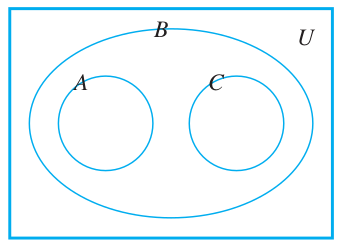
\includegraphics[scale=0.5]{../images/6.1.14.a.png}
\end{figure}
\end{proof}

\subsubsection{(b)}
\(C \subseteq A, B \cap C = \es\)

\begin{proof}
\begin{figure}[ht!]
\centering
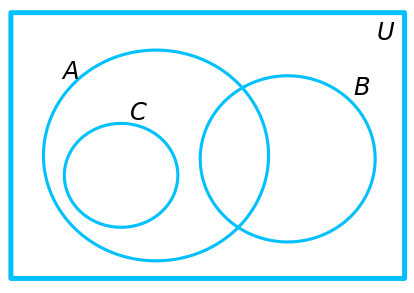
\includegraphics[scale=0.4]{../images/6.1.14.b.png}
\end{figure}
\end{proof}

\subsection{Exercise 15}
In each of the following, draw a Venn diagram for sets $A, B$, and $C$ that satisfy the given conditions.

\subsubsection{(a)}
\(A \cap B = \es, A \subseteq C, C \cap B \neq \es\)

\begin{proof}
\begin{figure}[ht!]
\centering
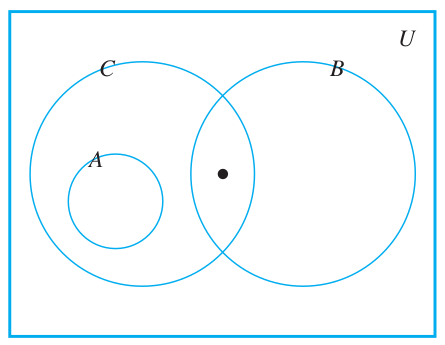
\includegraphics[scale=0.4]{../images/6.1.15.a.png}
\end{figure}
\end{proof}

\subsubsection{(b)}
\(A \subseteq B, C \subseteq B, A \cap C \neq \es\)

\begin{proof}
\begin{figure}[ht!]
\centering
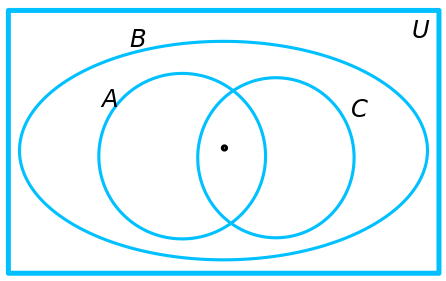
\includegraphics[scale=0.4]{../images/6.1.15.b.png}
\end{figure}
\end{proof}

\subsubsection{(c)}
\(A \cap B \neq \es, B \cap C \neq \es, A \cap C = \es, A \nsubseteq B, C \nsubseteq B\)

\begin{proof}
\begin{figure}[ht!]
\centering
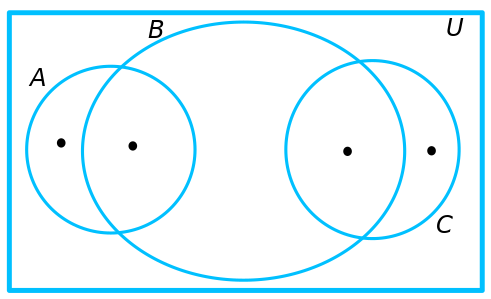
\includegraphics[scale=0.4]{../images/6.1.15.c.png}
\end{figure}
\end{proof}

\subsection{Exercise 16}
Let \(A = \{a, b, c\}, B = \{b, c, d\}, C = \{b, c, e\}\).

\subsubsection{(a)}
Find \(A \cup (B \cap C), (A \cup B) \cap C\), and \((A \cup B) \cap (A \cup C)\). Which of these sets are equal?

\begin{proof}
\(A \cup (B \cap C ) = \{a, b, c\}, (A \cup B) \cap C =
\{b, c\}\), 
and \((A \cup B) \cap (A \cup C ) = \{a, b, c, d\} \cap \{a, b, c, e\} = \{a, b, c\}\). 
Hence \(A \cup (B \cap C ) = (A \cup B) \cap (A \cup C).\)
\end{proof}

\subsubsection{(b)}
Find \(A \cap (B \cup C), (A \cap B) \cap C\), and \((A \cap B) \cup (A \cap C)\). Which of these sets are equal?

\begin{proof}
\(A \cap (B \cup C ) = \{b, c\}, (A \cap B) \cap C =
\{b, c\}\), 
and \((A \cap B) \cup (A \cap C ) = \{b, c\} \cup \{b, c\} = \{b, c\}\). 
Hence all three sets are equal.
\end{proof}

\subsubsection{(c)}
Find \((A - B) - C\) and \(A - (B - C)\). Are these sets equal?

\begin{proof}
\((A - B) - C = \{a\} - \{b, c, e\} = \{a\}\) and \(A - (B - C) = \{a, b, c\} - \{d\} = \{a, b, c\}\).
The sets are not equal.
\end{proof}

\subsection{Exercise 17}
\begin{figure}[ht!]
\centering
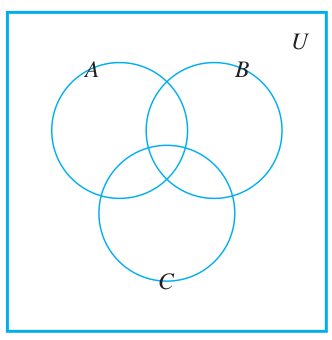
\includegraphics[scale=0.3]{../images/6.1.17.png}
\end{figure}
Consider the Venn diagram. For each of (a)-(f), copy the diagram and shade the region corresponding to the indicated set.

\subsubsection{(a)}
$A \cap B$

\begin{proof}
\begin{figure}[ht!]
\centering
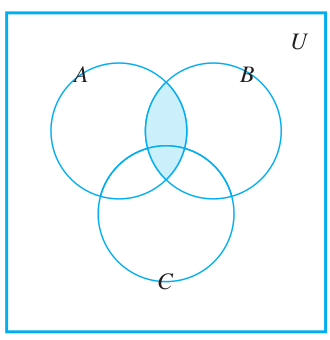
\includegraphics[scale=0.3]{../images/6.1.17.a.png}
\end{figure}
\end{proof}

\subsubsection{(b)}
$B \cup C$

\begin{proof}
\begin{figure}[ht!]
\centering
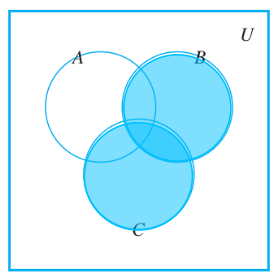
\includegraphics[scale=0.4]{../images/6.1.17.b.png}
\end{figure}
\end{proof}

\subsubsection{(c)}
$A^c$

\begin{proof}
\begin{figure}[ht!]
\centering
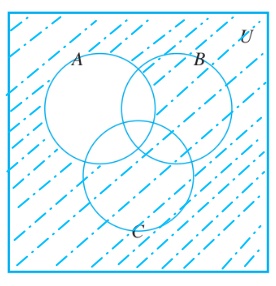
\includegraphics[scale=0.4]{../images/6.1.17.c.png}
\end{figure}
\end{proof}

\subsubsection{(d)}
$A - (B \cup C)$

\begin{proof}
\begin{figure}[ht!]
\centering
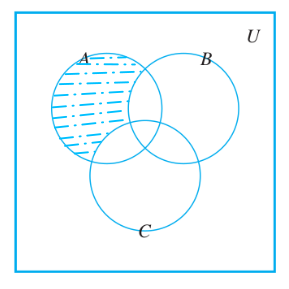
\includegraphics[scale=0.4]{../images/6.1.17.d.png}
\end{figure}
\end{proof}

\subsubsection{(e)}
$(A \cup B)^c$

\begin{proof}
\begin{figure}[ht!]
\centering
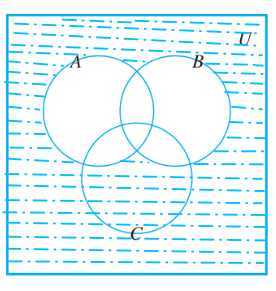
\includegraphics[scale=0.4]{../images/6.1.17.e.png}
\end{figure}
\end{proof}

\subsubsection{(f)}
$A^c \cap B^c$

\begin{proof}
Same as (e).
\end{proof}

\subsection{Exercise 18}

\subsubsection{(a)}
Is the number 0 in $\es$? Why?

\begin{proof}
The number 0 is not in $\es$ because $\es$ has no elements.
\end{proof}

\subsubsection{(b)}
Is $\es = \{\es\}$? Why?

\begin{proof}
No. The left-hand set is the empty set; it does not have any elements. The right-hand set is a set with one element, namely $\es$.
\end{proof}

\subsubsection{(c)}
Is $\es \in \{\es\}$? Why?

\begin{proof}
Yes. The left-hand side is the empty set; the right-hand side is a set with one element, namely $\es$. So the left-
hand side is an element of the right-hand side.
\end{proof}

\subsubsection{(d)}
Is $\es \in \es$? Why?

\begin{proof}
$\es$ is not in $\es$ because $\es$ has no elements.
\end{proof}

\subsection{Exercise 19}
Let \(A_i = \{i, i^2\}\) for each integer \(i = 1, 2, 3, 4\).

\subsubsection{(a)}
\(A_1 \cup A_2 \cup A_3 \cup A_4 = ?\)

\begin{proof}
\(A_1 = \{1, 1^2\} = \{1\}, A_2 = \{2, 2^2\} = \{2, 4\}, A_3 = \{3, 3^2\} = \{3, 9\}, A_4 = \{4, 4^2\} = \{4, 16\}\)

\(A_1 \cup A_2 \cup A_3 \cup A_4 = \{1\} \cup \{2, 4\} \cup \{3, 9\} \cup \{4, 16\} = \{1, 2, 3, 4, 9, 16\}\)
\end{proof}

\subsubsection{(b)}
\(A_1 \cap A_2 \cap A_3 \cap A_4 = ?\)

\begin{proof}
\(A_1 \cap A_2 \cap A_3 \cap A_4 = \{1\} \cap \{2, 4\} \cap \{3, 9\} \cap \{4, 16\} = \es\)
\end{proof}

\subsubsection{(c)}
Are \(A_1, A_2, A_3, A_4\) mutually disjoint? Explain.

\begin{proof}
\(A_1, A_2, A_3, A_4\) are not mutually disjoint, because \(A_2 \cap A_4 = \{4\} \neq \es\).
\end{proof}

\subsection{Exercise 20}
Let \(B_i = \{x \in \R \, | \, 0 \leq x \leq i\}\) for each integer \(i = 1, 2, 3, 4\).

\subsubsection{(a)}
\(B_1 \cup B_2 \cup B_3 \cup B_4 = ?\)

\begin{proof}
\(B_1 \cup B_2 \cup B_3 \cup B_4 = B_4 = [0, 4]\)
\end{proof}

\subsubsection{(b)}
\(B_1 \cap B_2 \cap B_3 \cap B_4 = ?\)

\begin{proof}
\(B_1 \cap B_2 \cap B_3 \cap B_4 = B_1 = [0, 1]\)
\end{proof}

\subsubsection{(c)}
Are \(B_1, B_2, B_3, B_4\) mutually disjoint? Explain.

\begin{proof}
No, because for example \(B_1 \cap B_2 = B_1 \neq \es\).
\end{proof}

\subsection{Exercise 21}
Let \(C_i = \{-i, i\}\) for each nonnegative integer $i$.

\subsubsection{(a)}
\(\dps \bigcup_{i=0}^{4}C_i = ?\)

\begin{proof}
\(C_0 = \{0, -0\} = \{0\}, C_1 = \{1, -1\}, C_2 = \{2, -2\}, C_3 = \{3, -3\}, C_4 = \{4, -4\}\)

\(\dps \bigcup_{i=0}^{4}C_i = \{-4, -3, -2, -1, 0, 1, 2, 3, 4\}\)
\end{proof}

\subsubsection{(b)}
\(\dps \bigcap_{i=0}^{4}C_i = ?\)

\begin{proof}
\(\dps \bigcap_{i=0}^{4}C_i = \{0\} \cap \{1, -1\} \cap \{2, -2\} \cap \{3, -3\} \cap \{4, -4\} = \es\)
\end{proof}

\subsubsection{(c)}
Are \(C_0, C_1, C_2, \ldots\) mutually disjoint? Explain.

\begin{proof}
$C_0, C_1, C_2, \ldots$ are mutually disjoint because no two of the sets have any elements in common.
\end{proof}

\subsubsection{(d)}
\(\dps \bigcup_{i=0}^{n}C_i = ?\)

\begin{proof}
\(\dps \bigcup_{i=0}^{n}C_i = \{-n, -(n-1), \ldots, -2, -1, 0, 1, 2, \ldots, n-1, n\}\)
\end{proof}

\subsubsection{(e)}
\(\dps \bigcap_{i=0}^{n}C_i = ?\)

\begin{proof}
\(\dps \bigcap_{i=0}^{n}C_i = \es\)
\end{proof}

\subsubsection{(f)}
\(\dps \bigcup_{i=0}^{\infty}C_i = ?\)

\begin{proof}
\(\dps \bigcup_{i=0}^{\infty}C_i = \Z\), the set of all integers
\end{proof}

\subsubsection{(g)}
\(\dps \bigcap_{i=0}^{\infty}C_i = ?\)

\begin{proof}
\(\dps \bigcap_{i=0}^{\infty}C_i = \es\)
\end{proof}

\subsection{Exercise 22}
Let \(D_i = \{x \in \R \,|\, -i \leq x \leq i\} = [-i, i]\) for each nonnegative integer $i$.

\subsubsection{(a)}
\(\dps \bigcup_{i=0}^{4}D_i = ?\)

\begin{proof}
\(D_0 = [-0, 0] = \{0\}, D_1 = [-1, 1], D_2 = [-2, 2], D_3 = [-3, 3], D_4 = [-4, 4]\)

\(\dps \bigcup_{i=0}^{4}D_i = \{0\} \cup [-1, 1] \cup [-2, 2] \cup [-3, 3] \cup [-4, 4] = [-4, 4]\)
\end{proof}

\subsubsection{(b)}
\(\dps \bigcap_{i=0}^{4}D_i = ?\)

\begin{proof}
\(\dps \bigcap_{i=0}^{4}D_i = \{0\} \cap [-1, 1] \cap [-2, 2] \cap [-3, 3] \cap [-4, 4] = \{0\}\)
\end{proof}

\subsubsection{(c)}
Are \(D_0, D_1, D_2, \ldots\) mutually disjoint? Explain.

\begin{proof}
$D_0, D_1, D_2, \ldots,$ are not mutually disjoint. In fact, each \(D_k \subseteq D_{k+1}\).
\end{proof}

\subsubsection{(d)}
\(\dps \bigcup_{i=0}^{n}D_i = ?\)

\begin{proof}
\(\dps \bigcup_{i=0}^{n}D_i = [-n, n]\)
\end{proof}

\subsubsection{(e)}
\(\dps \bigcap_{i=0}^{n}D_i = ?\)

\begin{proof}
\(\dps \bigcap_{i=0}^{n}D_i = \{0\}\)
\end{proof}

\subsubsection{(f)}
\(\dps \bigcup_{i=0}^{\infty}D_i = ?\)

\begin{proof}
\(\dps \bigcup_{i=0}^{\infty}D_i = \R\), the set of all real numbers
\end{proof}

\subsubsection{(g)}
\(\dps \bigcap_{i=0}^{\infty}D_i = ?\)

\begin{proof}
\(\dps \bigcap_{i=0}^{\infty}D_i = \{0\}\)
\end{proof}

\subsection{Exercise 23}
Let \(V_i = \{x \in \R \,|\, -\frac{1}{i} \leq x \leq \frac{1}{i}\} = [-\frac{1}{i}, \frac{1}{i}]\) 
for each positive integer $i$.

\subsubsection{(a)}
\(\dps \bigcup_{i=1}^{4}V_i = ?\)

\begin{proof}
\(\dps \bigcup_{i=1}^{4}V_i = V_1 = [-1, 1]\)
\end{proof}

\subsubsection{(b)}
\(\dps \bigcap_{i=1}^{4}V_i = ?\)

\begin{proof}
\(\dps \bigcap_{i=1}^{4}V_i = V_4 = \left[-\frac{1}{4}, \frac{1}{4}\right]\)
\end{proof}

\subsubsection{(c)}
Are \(V_1, V_2, V_3, \ldots\) mutually disjoint? Explain.

\begin{proof}
$V_1, V_2, V_3, \ldots,$ are not mutually disjoint. In fact, each \(V_{k+1} \subseteq V_k\).
\end{proof}

\subsubsection{(d)}
\(\dps \bigcup_{i=1}^{n}V_i = ?\)

\begin{proof}
\(\dps \bigcup_{i=1}^{n}V_i = V_1 = [-1, 1]\)
\end{proof}

\subsubsection{(e)}
\(\dps \bigcap_{i=1}^{n}V_i = ?\)

\begin{proof}
\(\dps \bigcap_{i=1}^{n}V_i = V_n = \left[-\frac{1}{n}, \frac{1}{n}\right]\)
\end{proof}

\subsubsection{(f)}
\(\dps \bigcup_{i=1}^{\infty}V_i = ?\)

\begin{proof}
\(\dps \bigcup_{i=1}^{\infty}V_i = V_1 = [-1, 1]\)
\end{proof}

\subsubsection{(g)}
\(\dps \bigcap_{i=1}^{\infty}V_i = ?\)

\begin{proof}
\(\dps \bigcap_{i=1}^{\infty}V_i = \{0\}\)
\end{proof}

\subsection{Exercise 24}
Let \(W_i = \{x \in \R \,|\, i < x\} = (i, \infty)\) for each nonnegative integer $i$.

\subsubsection{(a)}
\(\dps \bigcup_{i=0}^{4}W_i = ?\)

\begin{proof}
\(\dps \bigcup_{i=0}^{4}W_i = W_0 = (0, \infty)\)
\end{proof}

\subsubsection{(b)}
\(\dps \bigcap_{i=0}^{4}W_i = ?\)

\begin{proof}
\(\dps \bigcap_{i=0}^{4}W_i = W_4 = (4, \infty)\)
\end{proof}

\subsubsection{(c)}
Are \(W_0, W_1, W_2, \ldots\) mutually disjoint? Explain.

\begin{proof}
$W_0, W_1, W_2, \ldots,$ are not mutually disjoint. In fact, each \(W_{k+1} \subseteq W_k\).
\end{proof}

\subsubsection{(d)}
\(\dps \bigcup_{i=0}^{n}W_i = ?\)

\begin{proof}
\(\dps \bigcup_{i=0}^{n}W_i = W_0 = (0, \infty)\)
\end{proof}

\subsubsection{(e)}
\(\dps \bigcap_{i=0}^{n}W_i = ?\)

\begin{proof}
\(\dps \bigcap_{i=0}^{n}W_i = W_n = (n, \infty)\)
\end{proof}

\subsubsection{(f)}
\(\dps \bigcup_{i=0}^{\infty}W_i = ?\)

\begin{proof}
\(\dps \bigcup_{i=0}^{\infty}W_i = W_0 = (0, \infty)\)
\end{proof}

\subsubsection{(g)}
\(\dps \bigcap_{i=0}^{\infty}W_i = ?\)

\begin{proof}
\(\dps \bigcap_{i=0}^{\infty}W_i = \es\)
\end{proof}

\subsection{Exercise 25}
Let \(R_i = \{x \in \R \,|\, 1 \leq x \leq 1 + \frac{1}{i}\} = \left[1, 1 + \frac{1}{i}\right]\) 
for each positive integer $i$.

\subsubsection{(a)}
\(\dps \bigcup_{i=1}^{4}R_i = ?\)

\begin{proof}
\(\dps \bigcup_{i=1}^{4}R_i = R_1 = [1, 2]\)
\end{proof}

\subsubsection{(b)}
\(\dps \bigcap_{i=1}^{4}R_i = ?\)

\begin{proof}
\(\dps \bigcap_{i=1}^{4}R_i = R_4 = \left[1, \frac{5}{4}\right]\)
\end{proof}

\subsubsection{(c)}
Are \(R_1, R_2, R_3, \ldots\) mutually disjoint? Explain.

\begin{proof}
No, in fact each \(R_{k+1} \subseteq R_k\).
\end{proof}

\subsubsection{(d)}
\(\dps \bigcup_{i=1}^{n}R_i = ?\)

\begin{proof}
\(\dps \bigcup_{i=1}^{n}R_i = R_1 = [1, 2]\)
\end{proof}

\subsubsection{(e)}
\(\dps \bigcap_{i=1}^{n}R_i = ?\)

\begin{proof}
\(\dps \bigcap_{i=1}^{n}R_i = R_n = \left[1, 1+\frac{1}{n}\right]\)
\end{proof}

\subsubsection{(f)}
\(\dps \bigcup_{i=1}^{\infty}R_i = ?\)

\begin{proof}
\(\dps \bigcup_{i=1}^{\infty}R_i = R_1 = [1, 2]\)
\end{proof}

\subsubsection{(g)}
\(\dps \bigcap_{i=1}^{\infty}R_i = ?\)

\begin{proof}
\(\dps \bigcap_{i=1}^{\infty}R_i = \{1\}\)
\end{proof}

\subsection{Exercise 26}
Let \(S_i = \{x \in \R \,|\, 1 < x < 1 + \frac{1}{i}\} = \left(1, 1 + \frac{1}{i}\right)\) 
for each positive integer $i$.

\subsubsection{(a)}
\(\dps \bigcup_{i=1}^{4}S_i = ?\)

\begin{proof}
\(\dps \bigcup_{i=1}^{4}S_i = S_1 = (1, 2)\)
\end{proof}

\subsubsection{(b)}
\(\dps \bigcap_{i=1}^{4}S_i = ?\)

\begin{proof}
\(\dps \bigcap_{i=1}^{4}S_i = S_4 = (1, 5/4)\)
\end{proof}

\subsubsection{(c)}
Are \(S_0, S_1, S_2, \ldots\) mutually disjoint? Explain.

\begin{proof}
No, in fact each \(S_{k+1} \subseteq S_k\).
\end{proof}

\subsubsection{(d)}
\(\dps \bigcup_{i=1}^{n}S_i = ?\)

\begin{proof}
\(\dps \bigcup_{i=1}^{n}S_i = S_1 = (1, 2)\)
\end{proof}

\subsubsection{(e)}
\(\dps \bigcap_{i=1}^{n}S_i = ?\)

\begin{proof}
\(\dps \bigcap_{i=1}^{n}S_i = S_n = (1, \frac{n+1}{n})\)
\end{proof}

\subsubsection{(f)}
\(\dps \bigcup_{i=1}^{\infty}S_i = ?\)

\begin{proof}
\(\dps \bigcup_{i=1}^{\infty}S_i = S_1 = (1, 2)\)
\end{proof}

\subsubsection{(g)}
\(\dps \bigcap_{i=1}^{\infty}S_i = ?\)

\begin{proof}
\(\dps \bigcap_{i=1}^{\infty}S_i = (1, 1) = \es\)
\end{proof}

\subsection{Exercise 27}

\subsubsection{(a)}
Is \(\{\{a, d, e\}, \{b, c\}, \{d, f\}\}\) a partition of
\(\{a, b, c, d, e, f\}\)?

\begin{proof}
No. The element $d$ is in two of the sets.
\end{proof}

\subsubsection{(b)}
Is \(\{\{w, x, v\}, \{u, y, q\}, \{p, z\}\}\) a partition of \(\{p, q, u, v, w, x, y, z\}\)?

\begin{proof}
Yes.
\end{proof}

\subsubsection{(c)}
Is \(\{\{5, 4\}, \{7, 2\}, \{1, 3, 4\}, \{6, 8\}\}\) a partition of \(\{1, 2, 3, 4, 5, 6, 7, 8\}\)?

\begin{proof}
No. The element $4$ is in two of the sets.
\end{proof}

\subsubsection{(d)}
Is \(\{\{3, 7, 8\}, \{2, 9\}, \{1, 4, 5\}\}\) a partition of \(\{1, 2, 3, 4, 5, 6, 7, 8, 9\}\)?

\begin{proof}
No. None of the sets contains 6.
\end{proof}

\subsubsection{(e)}
Is \(\{\{1, 5\}, \{4, 7\}, \{2, 8, 6, 3\}\}\) a partition of \(\{1, 2, 3, 4, 5, 6, 7, 8\}\)?

\begin{proof}
Yes.
\end{proof}

\subsection{Exercise 28}
Let $E$ be the set of all even integers and $O$ the set of all odd integers. Is \(\{E, O\}\) a partition of $\Z$, the set of all integers? Explain your answer.

\begin{proof}
Yes. Every integer is either even or odd, and no integer is both even and odd.
\end{proof}

\subsection{Exercise 29}
Let $\R$ be the set of all real numbers. Is $\{R^+, R^-, \{0\}\}$ a partition of $\R$? Explain your answer.

\begin{proof}
Yes. Every real number is either positive or negative or zero, and no real number is both positive and negative, and 
zero is neither negative nor positive (so the three sets are mutually disjoint).
\end{proof}

\subsection{Exercise 30}
Let $Z$ be the set of all integers and let
\begin{center}
\begin{tabular}{rcl}
$A_1$ & = & \(\{n \in \Z \, | \, n = 4k \text{ for some integer } k\}\) \\
$A_2$ & = & \(\{n \in \Z \, | \, n = 4k + 1 \text{ for some integer } k\}\) \\
$A_3$ & = & \(\{n \in \Z \, | \, n = 4k + 2 \text{ for some integer } k\}\) \\
$A_4$ & = & \(\{n \in \Z \, | \, n = 4k + 3 \text{ for some integer } k\}\) 
\end{tabular}
\end{center}
Is \(\{A_0, A_1, A_2, A_3\}\) a partition of $\Z$? Explain your answer.

\begin{proof}
Yes. These sets are mutually disjoint, and by the quotient-remainder theorem, every integer has exactly one of the 
forms \(n = 4k\) or \(n = 4k+1\) or \(n = 4k+2\) or \(n = 4k+3\).
\end{proof}

\subsection{Exercise 31}
Suppose \(A = \{1, 2\}, B = \{2, 3\}\). Find each of the following:

\subsubsection{(a)}
\(\ps(A \cap B)\)

\begin{proof}
\(A \cap B = \{2\}\), so \(\ps(A \cap B) = \{\es, \{2\}\}\).
\end{proof}

\subsubsection{(b)}
\(\ps(A)\)

\begin{proof}
\(A = \{1, 2\}\), so \(\ps(A) = \{\es, \{1\}, \{2\}, \{1, 2\}\}\).
\end{proof}

\subsubsection{(c)}
\(\ps(A \cup B)\)

\begin{proof}
\(A \cup B = \{1, 2, 3\}\), so \(\ps(A \cup B) = \{\es, \{1\}, \{2\}, \{3\}, \{1, 2\}, \{1, 3\}, \{2, 3\}, \{1, 2, 3\}\}\).
\end{proof}

\subsubsection{(d)}
\(\ps(A \times B)\)

\begin{proof}
\(A \times B = \{(1, 2), (1, 3), (2, 2), (2, 3)\}\), so \(\ps(A\times B)=\{\es, \{(1, 2)\},\{(1, 3)\},\{(2, 2)\},\)

\(\{(2, 3)\}, \{(1, 2), (1, 3)\}, \{(1, 2), (2, 2)\}, \{(1, 2), (2, 3)\}, \{(1, 3), (2, 2)\}, \{(1, 3), (2, 3)\}, \)

\(\{(2, 2), (2, 3)\}, \{(1, 2), (1, 3), (2, 2)\}, \{(1, 2), (1, 3), (2, 3)\}, \{(1, 2), (2, 2), (2, 3)\}, \)

\(\{(1, 3), (2, 2), (2, 3)\}, \{(1, 2), (1, 3), (2, 2), (2, 3)\}\}\).
\end{proof}

\subsection{Exercise 32}

\subsubsection{(a)}
Suppose \(A = \{1\}, B = \{u, v\}\). Find \(\ps(A \times B)\).

\begin{proof}
\(\ps(A \times B) = \{\es, \{(1, u)\}, \{(1, v)\}, \{(1, u), (1, v)\}\}\)
\end{proof}

\subsubsection{(b)}
Suppose \(X = \{a, b\}, Y = \{x, y\}\). Find \(\ps(X \times Y)\).

\begin{proof}
\(X \times Y = \{(a, x), (a, y), (b, x), (b, y)\}\)

\(\ps(X \times Y) = \{\es, \{(a, x)\}, \{(a, y)\}, \{(b, x)\}, \{(b, y)\}, \{(a, x), (a, y)\}, \{(a, x), (b, x)\},\)

\(\{(a, x), (b, y)\}, \{(a, y), (b, x)\}, \{(a, y), (b, y)\}, \{(b, x), (b, y)\}, \{(a, x), (a, y), (b, x)\},\) 

\(\{(a, x), (a, y), (b, y)\}, \{(a, x), (b, x), (b, y)\}, \{(a, y), (b, x), (b, y)\},\) 

\(\{(a, x), (a, y), (b, x), (b, y)\}\}\)
\end{proof}

\subsection{Exercise 33}

\subsubsection{(a)}
Find \(\ps(\es)\).

\begin{proof}
\(\ps(\es) = \{\es\}\)
\end{proof}

\subsubsection{(b)}
Find \(\ps(\ps(\es))\).

\begin{proof}
\(\ps(\ps(\es)) = \ps(\{\es\}) = \{\es, \{\es\}\}\)
\end{proof}

\subsubsection{(c)}
Find \(\ps(\ps(\ps(\es)))\).

\begin{proof}
\(\ps(\ps(\ps(\es))) = \ps(\{\es, \{\es\}\}) = \{\es, \{\es\}, \{\{\es\}\}, \{\es, \{\es\}\}\}\)
\end{proof}

\subsection{Exercise 34}
Let \(A_1 = \{1\}, A_2 = \{u, v\}, A_3 = \{m, n\}\). Find each of the following sets:

\subsubsection{(a)}
$A_1 \cup (A_2 \times A_3)$

\begin{proof}
\(A_1 \cup (A_2 \times A_3) = \{1\} \cup \{(u, m), (u, n), (v, m), (v, n)\}\)

\(= \{1, (u, m), (u, n), (v, m), (v, n)\}\)
\end{proof}

\subsubsection{(b)}
$(A_1 \cup A_2) \times A_3$

\begin{proof}
\((A_1 \cup A_2) \times A_3 = \{1, u, v\} \times \{m, n\} = \{(1, m), (1, n), (u, m), (u, n), (v, m), (v, n)\}\)
\end{proof}

\subsection{Exercise 35}
Let \(A = \{a, b\}, B = \{1, 2\}, C = \{2, 3\}\). Find each of the following sets.

\subsubsection{(a)}
$A \times (B \cup C)$

\begin{proof}
\(A \times (B \cup C) = \{a, b\} \times \{1, 2, 3\}\ = \{(a, 1), (a, 2), (a, 3), (b, 1), (b, 2), (b, 3)\}\)
\end{proof}

\subsubsection{(b)}
$(A \times B) \cup (A \times C)$

\begin{proof}
\((A \times B) \cup (A \times C) = \{(a, 1), (a, 2), (b, 1), (b, 2), (a, 2), (a, 3), (b, 2), (b, 3)\}\) 

\(= \{(a, 1), (a, 2), (b, 1), (b, 2), (a, 3), (b, 3)\}\)
\end{proof}

\subsubsection{(c)}
$A \times (B \cap C)$

\begin{proof}
\(A \times (B \cap C) = \{a, b\} \times \{2\}\ = \{(a, 2), (b, 2)\}\)
\end{proof}

\subsubsection{(d)}
$(A \times B) \cap (A \times C)$

\begin{proof}
\((A \times B) \cap (A \times C) = \{(a, 1), (a, 2), (b, 1), (b, 2)\} \cap \{(a, 2), (a, 3), (b, 2), (b, 3)\}\) 

\(= \{(a, 2), (b, 2)\}\)
\end{proof}

\subsection{Exercise 36}
Trace the action of Algorithm 6.1.1 on the variables $i, j, found$, and $answer$ for $m = 3, n = 3$, and sets $A$ and 
$B$ represented as the arrays \(a[1] = u, a[2] = v, a[3] = w, b[1] = w, b[2] = u, b[3] = v\).

\begin{proof}
\begin{figure}[ht!]
\centering
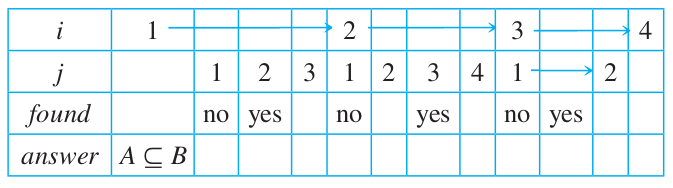
\includegraphics[scale=0.5]{../images/6.1.36.png}
\end{figure}
\end{proof}

\subsection{Exercise 37}
Trace the action of Algorithm 6.1.1 on the variables $i, j, found$, and $answer$ for $m = 4, n = 4$, and sets $A$ and 
$B$ represented as the arrays \(a[1] = u, a[2] = v, a[3] = w, a[4] = x, b[1] = r, b[2] = u, b[3] = y, b[4] = z\).

\begin{proof}
\begin{center}
\arrayrulecolor{cyan} % change rule color
\begin{tabular}{|l|c|c|c|c|c|c|c|c|}
\hline
{\bf i} & 1 & & & & 2 & & & \\
\hline
{\bf j} & 1 & 2 & 3 & 4 & 1 & 2 & 3 & 4 \\
\hline
{\bf found} & no & yes & & & no & & & \\
\hline
{\bf answer} & \(A \subseteq B\) & & & & & & & \(A \nsubseteq B\) \\
\hline
\end{tabular}
\arrayrulecolor{black} % change it back!
\end{center}
\end{proof}

\subsection{Exercise 38}
Write an algorithm to determine whether a given element $x$ belongs to a given set that is represented as the array 
\(a[1], a[2], \ldots, a[n]\).

\begin{tcolorbox}[colframe=cyan]
{\bf \cy Algorithm: Testing whether $x \in A$} 

{\cy Input:} $x$ (an element), $n$ (a positive integer), \(a[1], \ldots, a[n]\) (a one-dimensional array representing 
the set $A$).

{\cy Algorithm Body:}
\begin{tabbing}
\(i \coloneqq 1, answer \coloneqq\) ``\(x \notin A\)'' \\
{\bf while} \= (\(i \leq n\) and \(answer =\) ``\(x \notin A\)'') \\
            \> {\bf if} \(x = a[i]\) {\bf then} \(answer = \) ``\(x \in A\)'' \\
            \> \(i \coloneqq i + 1\) \\
{\bf end while}
\end{tabbing}
{\cy Output:} {\it answer [a string]}
\end{tcolorbox}

\end{document}
